%% CEUR-WS working note. Single column: the CEURART template explicitly warns
%% "Do not use twocolumn for papers submitted to CEUR-WS!"
\documentclass{ceurart}

\sloppy

\usepackage{booktabs}
\usepackage{graphicx}
\usepackage{tikz}
\usetikzlibrary{arrows.meta, positioning, fit, backgrounds, calc}
\usepackage{amsmath}
\usepackage{multirow}

\begin{document}

\copyrightyear{2026}
\copyrightclause{Copyright \copyright{} 2026 for this paper by its authors.
  Use permitted under Creative Commons License Attribution 4.0
  International (CC BY 4.0).}

\conference{Forum for Information Retrieval Evaluation, December 17--20, 2026,
  Indian Statistical Institute, Kolkata, India}

%% Per the organisers' guidelines the title carries neither a team name nor the
%% track name, and the author name carries no prefix.
\title{Diagnosing the Evaluation Distribution: Argument-Taxonomy Distillation
  and an English Pivot for Climate Stance Detection in Hindi and Bengali}

\author[1]{Koushik Deb}[
  %% \string_ gives a catcode-12 underscore: prints correctly and survives
  %% hyperref writing it into the mailto: URL (a plain \_ errors there).
  email=koushik\string_phd21@iiitkalyani.ac.in,
  orcid=0000-0001-7902-4387,
]
\address[1]{Indian Institute of Information Technology Kalyani, Kalyani,
  West Bengal, 741235, India}

\begin{abstract}
  We describe our submission to a shared task on detecting the stance of Hindi
  and Bengali YouTube comments towards the claim \emph{``climate change and
  global warming is a serious concern''}, given only English training
  resources. Our central finding is procedural rather than architectural: the
  decisive step was measuring the evaluation data before choosing a transfer
  strategy. Inspection of the released files shows that they consist of
  \emph{machine-translated English} comments---no romanised code-mixing, no
  emoji, three mentions of India across 500 Bengali comments, and recurring
  arguments about a science communicator's credentials and the ``97\,\%
  consensus'' figure. Building for that distribution instead of for organic
  Indic social media reversed our design. We formalise a 27-node
  climate-argument taxonomy that extends the CARDS scheme with an
  India-specific branch and an explicit \textsc{None} inventory, and use it as
  a generative schema, as auxiliary supervision, and as an annotation
  scaffold. We distil a nine-model large-language-model panel over the
  unlabelled evaluation set into compact encoders. Finally we exploit the
  forensic finding a second time by back-translating the evaluation set into
  English and classifying with an English-only encoder, which sidesteps the
  cross-lingual problem rather than solving it; this is worth $+0.10$ macro-F1
  over the best multilingual configuration, verified by a paired test over 300
  shared data splits. Our submitted system attains macro-F1 $0.922$ (Hindi)
  and $0.915$ (Bengali) on a held-out development set. We state clearly that
  those development labels come from a language-model judge panel rather than
  human annotation, and we report both the reliability evidence and its
  limits. We also document four negative results, including a methodological
  trap in which comparing ensemble strategies by unpaired means overstated one
  apparent gain and reversed the sign of another.
\end{abstract}

\begin{keywords}
  stance detection \sep
  low-resource languages \sep
  Hindi \sep
  Bengali \sep
  knowledge distillation \sep
  argument mining \sep
  model calibration
\end{keywords}

\maketitle

%% ---------------------------------------------------------------------------
\section{Introduction}

Stance detection asks how a text positions itself with respect to a fixed
claim, which is distinct from sentiment: a furious comment and an approving one
can take the same stance, and a polite one can take none at all. Given a
YouTube comment in Hindi or Bengali, the task is to assign \textsc{Favour},
\textsc{Against}, or \textsc{None} with respect to the claim \emph{``climate
change and global warming is a serious concern''}. The organisers supply
English-only training resources and evaluate on Hindi and Bengali, so
cross-lingual transfer is the nominal challenge. Runs are ranked by macro-F1,
and more than eighty runs were submitted to the track.

Two properties of the task shaped our approach. First, macro-F1 weights every
class equally, so the \textsc{Against} class---about $15\,\%$ of the permitted
English pool---carries a full third of the score. A system that never
confidently predicts \textsc{Against} is arithmetically capped near $0.45$
however well it performs elsewhere. Second, and less obviously, the evaluation
data is not what the task description leads one to expect. We therefore begin
with a diagnostic rather than a model.

\paragraph{Contributions.}
\begin{enumerate}
  \item A forensic characterisation of the evaluation set
    (Section~\ref{sec:forensics}) establishing that it consists of
    machine-translated English comments, together with the four design
    decisions that follow.
  \item A 27-node climate-argument taxonomy (Section~\ref{sec:taxonomy})
    extending CARDS~\cite{coan2021} with an India-specific contrarian branch, a
    mirrored pro-climate branch, and an explicit \textsc{None} inventory, used
    in three distinct roles.
  \item An English-pivot classifier (Section~\ref{sec:pivot}) worth $+0.10$
    macro-F1 over the best multilingual system.
  \item Transductive panel distillation and macro-F1-aware calibration,
    each measured separately (Sections~\ref{sec:distil} and~\ref{sec:calib}).
  \item Four negative and methodological results
    (Section~\ref{sec:negative}) that we believe are more useful to report than
    a further architecture.
\end{enumerate}

%% ---------------------------------------------------------------------------
\section{Related Work}

Stance detection was established as a benchmark task by SemEval-2016 Task
6~\cite{mohammad2016}, and extended to unseen targets by zero-shot
formulations~\cite{allaway2020}. For climate discourse specifically, GWSD
provides English news sentences with crowd stance
annotations~\cite{luo2020}, and the CARDS scheme organises contrarian claims
into a hierarchy of super-claims and sub-claims~\cite{coan2021}, which we adopt
and extend.

Cross-lingual transfer for Indic languages typically relies on multilingual
encoders: XLM-R~\cite{conneau2020}, MuRIL~\cite{khanuja2021}, pre-trained on
Indian-language corpora including transliterated pairs, and
IndicBERTv2~\cite{doddapaneni2023}. An alternative reformulates
classification as entailment against a hypothesis~\cite{yin2019}, using
XNLI-trained models in multilingual settings~\cite{conneau2018xnli}; we include
this as a baseline. Surveys document rapid adoption of large language models
for stance detection~\cite{wang2024survey}, generally as direct predictors or
as annotators.

We instead use language models as a \emph{teacher}, following knowledge
distillation~\cite{hinton2015}: panel labels on unlabelled target data are
distilled into the compact encoder we actually submit, which keeps every run a
locally reproducible classifier rather than a live API call. Our projection
channel adapts a hybrid framework for multilingual zero-shot
classification~\cite{deb2026} aligning sentence embeddings with knowledge-graph
label embeddings; where that work uses ConceptNet~\cite{speer2017} we
substitute our task-specific taxonomy, and we retain its
Kolmogorov--Arnold~\cite{liu2024} alignment.

%% ---------------------------------------------------------------------------
\section{Task and Data}
\label{sec:data}

The evaluation data comprises two files of 500 comments each, for Hindi and
Bengali, with columns \texttt{ID} and \texttt{COMMENT} and identifiers
$1$--$500$ in both files. Runs are submitted as one file per language carrying
up to three classifier columns.

The permitted training resources are two English stance corpora:
\textbf{GWSD}~\cite{luo2020}, 2\,300 news sentences each annotated by eight
crowd workers, and \textbf{SemEval-2016 Task 6}~\cite{mohammad2016} restricted
to the target \emph{``Climate Change is a Real Concern''} (395 tweets). Other
public data, machine translation and synthetic generation are explicitly
permitted, and the organisers encourage making the training set more
appropriate for the task.

Merging and de-duplicating yields 2\,442 rows (\textsc{None} 1\,092,
\textsc{Favour} 983, \textsc{Against} 367). For GWSD we retain the full crowd
vote distribution rather than only the majority label: an 8--0 vote and a 5--3
vote are different training signals, and the soft target regularises the small
\textsc{Against} class at no cost. Mean GWSD annotator agreement is $0.72$.
Only $15.0\,\%$ of the pool is \textsc{Against}, and within the SemEval subset
just $3.8\,\%$ (15 of 395). Under macro-F1 this is not a detail but the
substance of the task.

%% ---------------------------------------------------------------------------
\section{Characterising the Evaluation Set}
\label{sec:forensics}

Before training any model we measured the released files.
Table~\ref{tab:forensics} summarises the result. Organic Indian YouTube
comments are short, emoji-dense and substantially Roman-script; these
comments are none of those things.

\begin{table}[t]
\centering
\caption{Measurements over all 1\,000 evaluation comments.}
\label{tab:forensics}
\begin{tabular}{lrr}
\toprule
Signal & Hindi & Bengali \\
\midrule
Comments naming one science communicator & 63 & 96 \\
Roman-script code-mixing & 0 & 0 \\
Comments containing any emoji & 0 & 0 \\
Comments mentioning India & 2 & 3 \\
Median length (characters) & 146 & 147 \\
\bottomrule
\end{tabular}
\end{table}

The register is uniformly formal and the arguments are drawn from a United
States-centric repertoire: attacks on a presenter's credentials
(\emph{``not a scientist, a mechanical engineer''}), disputes over the
``97\,\%'' consensus figure, channel-merchandise spam, creationist framing
(\emph{``why did God kill the dinosaurs''}), and comments indicating a school
assignment (\emph{``who else is here for online classes''}). Numerals appear
in Devanagari and Bengali digits and English names are transliterated. We
conclude that the evaluation set consists of English YouTube comments
machine-translated into Hindi and Bengali.

Matching the multiset of numerals per comment---normalised across Devanagari,
Bengali and ASCII digits---shows that the two language files are different
comment samples rather than translations of the same 500 English comments, so
no cross-file alignment shortcut exists.

\paragraph{Four consequences.}
This reverses the natural design. First, translate-test becomes the primary
channel rather than a fallback: back-translation recovers near-original
English, the native domain of GWSD, of SemEval, and of every strong English
encoder (Section~\ref{sec:pivot}). Second, one sentence of provenance context
in an annotation prompt resolves whole families of otherwise ambiguous items.
Third, synthetic data should imitate translationese---pure native script,
formal register, no emoji, transliterated names---rather than authentic Indian
slang. Fourth, the argument inventory to cover is the source community's, not
the target language's; our India-specific taxonomy branch, designed before
this measurement, accordingly became a minor slice, and we report it as an
ablation rather than as the centrepiece.

%% ---------------------------------------------------------------------------
\section{Argument Taxonomy}
\label{sec:taxonomy}

Cross-lingual stance transfer for climate discourse fails less because of
language mismatch than because of \emph{argument-inventory} mismatch. GWSD and
SemEval encode a United States contrarian idiom; translating them yields
fluent Hindi sentences about Al Gore, which is grammatically correct and
pedagogically useless. We therefore pivot through the argument rather than
through the language.

Our taxonomy contains 27 nodes---13 \textsc{Against}, 7 \textsc{Favour},
7 \textsc{None}---with 228 cue phrases across English, Hindi and Bengali. The
\textbf{CARDS branch} (6 nodes) follows Coan et al.~\cite{coan2021}: not
happening; not human-caused; impacts not harmful; solutions will not work;
science unreliable; and one node we added, \emph{attacks on the messenger},
which the measurements in Section~\ref{sec:forensics} showed to be among the
most frequent arguments actually present. The \textbf{India-specific
contrarian branch} (7 nodes) covers climate colonialism and whataboutism,
development-first arguments, local-weather naturalism, cyclical or religious
cosmology, media conspiracy, elite hypocrisy, and
population-rather-than-climate. The \textbf{pro-climate branch} (7 nodes) is
grounded in lived experience: floods and air quality, agricultural harm,
health, intergenerational duty, demands for action, support for mitigation,
and trust in science. The \textbf{\textsc{None} inventory} (7 nodes) covers
channel praise, pure questions, neutral factual statements, unrelated
politics, spam, ambivalence, and---again added after the
measurements---comments indicating a class assignment.

Two annotation traps are encoded explicitly, because they are where systems
and annotators most often diverge. \emph{Sentiment is not stance}:
\emph{``Shame on this government, they have destroyed our rivers!''} is
\textsc{Favour} despite maximally negative sentiment. \emph{Praise of the
video is not agreement with the claim}: \emph{``very informative, thank
you''} is \textsc{None} even under a climate-alarm video.

The taxonomy is used in three roles, and that triple use is what makes it a
contribution rather than a lexicon appendix: as a generative schema
(Section~\ref{sec:synth}), as auxiliary supervision
(Section~\ref{sec:encoder}), and as the reasoning scaffold in the annotation
prompt (Section~\ref{sec:distil}).

%% ---------------------------------------------------------------------------
\section{Method}

Figure~\ref{fig:pipeline} shows the full pipeline.

\begin{figure*}[t]
\centering
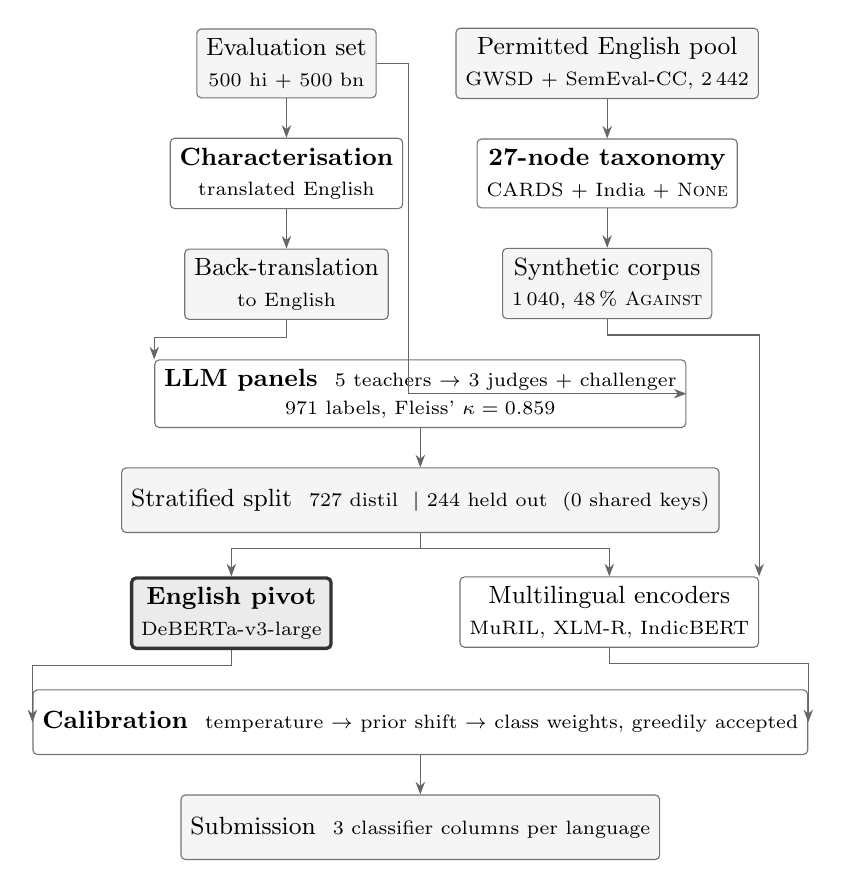
\begin{tikzpicture}[
  font=\small,
  node distance=3.2mm,
  box/.style={draw=black!55, rounded corners=1.6pt, align=center,
              inner sep=3.4pt, minimum height=8.2mm, fill=white},
  data/.style={box, fill=black!4},
  pivot/.style={box, very thick, draw=black!80, fill=black!8},
  ar/.style={-{Stealth[length=1.6mm]}, draw=black!60},
]
%% row 1 — inputs
\node[data] (test)  {Evaluation set\\\scriptsize 500 hi + 500 bn};
\node[data, right=10mm of test] (eng) {Permitted English pool\\\scriptsize GWSD + SemEval-CC, 2\,442};

%% forensics
\node[box, below=5mm of test] (foren) {\textbf{Characterisation}\\\scriptsize translated English};

%% taxonomy
\node[box, below=5mm of eng] (tax) {\textbf{27-node taxonomy}\\\scriptsize CARDS + India + \textsc{None}};

%% row 3
\node[data, below=5mm of foren] (bt) {Back-translation\\\scriptsize to English};
\node[data, below=5mm of tax] (synth) {Synthetic corpus\\\scriptsize 1\,040, 48\,\% \textsc{Against}};

%% panels
\node[box, below=5mm of bt, xshift=17mm] (panel)
  {\textbf{LLM panels}\ \ \scriptsize 5 teachers $\rightarrow$ 3 judges + challenger\\[-1pt]
   \scriptsize 971 labels, Fleiss' $\kappa=0.859$};

%% split
\node[data, below=5mm of panel] (split)
  {Stratified split\ \ \scriptsize 727 distil \ $|$\ 244 held out \ (0 shared keys)};

%% models
\node[pivot, below=5.5mm of split, xshift=-24mm] (deb)
  {\textbf{English pivot}\\\scriptsize DeBERTa-v3-large};
\node[box, below=5.5mm of split, xshift=24mm] (mult)
  {Multilingual encoders\\\scriptsize MuRIL, XLM-R, IndicBERT};

%% calibration + submission
\node[box, below=5mm of deb, xshift=24mm] (cal)
  {\textbf{Calibration}\ \ \scriptsize temperature $\rightarrow$ prior shift $\rightarrow$ class weights, greedily accepted};
\node[data, below=5mm of cal] (sub)
  {Submission\ \ \scriptsize 3 classifier columns per language};

\draw[ar] (test) -- (foren);
\draw[ar] (eng)  -- (tax);
\draw[ar] (foren) -- (bt);
\draw[ar] (tax)  -- (synth);
\draw[ar] (bt.south)    -- ++(0,-2.2mm) -| (panel.north west);
\draw[ar] (test.east) -- ++(4mm,0) |- (panel.east);
\draw[ar] (panel) -- (split);
\draw[ar] (split.south) -- ++(0,-2mm) -| (deb.north);
\draw[ar] (split.south) -- ++(0,-2mm) -| (mult.north);
\draw[ar] (synth.south) -- ++(0,-2mm) -| (mult.north east);
\draw[ar] (deb.south)  -- ++(0,-2mm) -| (cal.west);
\draw[ar] (mult.south) -- ++(0,-2mm) -| (cal.east);
\draw[ar] (cal) -- (sub);
\end{tikzpicture}
\caption{The pipeline. Characterising the evaluation set (upper left) is what
makes the English pivot available; everything downstream of it is a
consequence of that measurement rather than a prior design choice.}
\label{fig:pipeline}
\end{figure*}

\subsection{Taxonomy-conditioned synthetic augmentation}
\label{sec:synth}

We walk the product
$\text{node} \times \text{language} \times \text{script} \times
\text{register}$
and prompt a language model for realistic comments in each cell. Because the
stance is fixed by the cell, the corpus is class-balanced by construction.
Following Section~\ref{sec:forensics} we generate in translationese style. The
result is 1\,040 comments covering all 27 nodes, of which $48\,\%$ are
\textsc{Against}. Provenance columns (node, branch, language, register,
generator) are retained for ablation, and near-duplicates are removed by token
Jaccard similarity within each (node, language) cell.

Figure~\ref{fig:shift} shows why this matters, and contains an unplanned
validation. The permitted English pool is $15\,\%$ \textsc{Against}; the
synthetic corpus was deliberately built at $48\,\%$; and the evaluation set,
as later labelled by our judge panel, turned out to be $44\,\%$
\textsc{Against}. The synthetic distribution was therefore constructed to
match a target we had not yet measured, and landed within four points of it.

\begin{figure}[t]
\centering
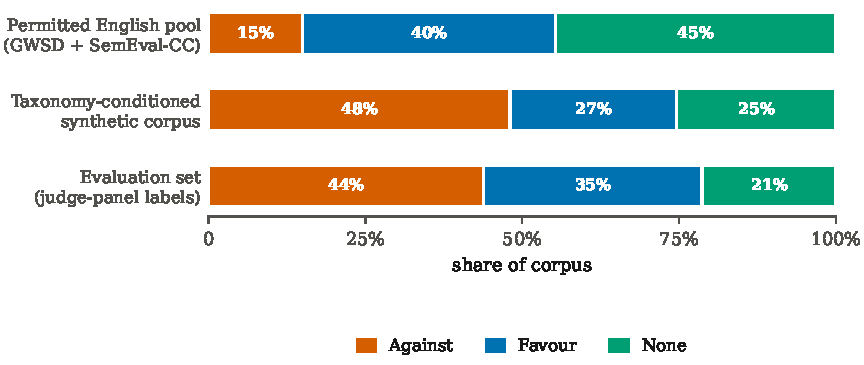
\includegraphics[width=\linewidth]{figures/fig_class_shift.pdf}
\caption{Class composition of the three corpora. The permitted training pool
is dominated by \textsc{None} and \textsc{Favour}; the evaluation set is
\textsc{Against}-heavy. Under macro-F1 this mismatch, not the language gap, is
what caps a naive system.}
\label{fig:shift}
\end{figure}

\subsection{Transductive panel distillation}
\label{sec:distil}

The entire \emph{unlabelled} evaluation set is available at inference time.
Using it is transduction, not leakage: no organiser-provided label is read at
any point. We run two disjoint panels over all 1\,000 comments.

A \textbf{teacher panel} of five inexpensive models from five different
laboratories labels every comment. Each model must name a taxonomy node
\emph{before} emitting a stance, which is chain-of-thought constrained to a
fixed and auditable vocabulary. A \textbf{judge panel} of three stronger
models then adjudicates, reading the Indic original together with its English
back-translation, with a fourth model adversarially challenging every proposed
label. Panels are disjoint by construction and the code refuses to run if any
model identifier appears in both roles.

\begin{table}[t]
\centering
\caption{Panel reliability. Teacher-panel $\kappa$ is reported per language.}
\label{tab:panels}
\begin{tabular}{lr}
\toprule
Measure & Value \\
\midrule
Teacher panel Fleiss' $\kappa$ (5 models) & 0.767 / 0.749 \\
Judge panel Fleiss' $\kappa$ (3 models) & \textbf{0.859} \\
Judge labels accepted (of 1\,000) & 971 \\
Adversarial overturn rate & 2.8\,\% \\
Teacher--judge agreement & 92.7\,\% \\
Teacher macro-F1 against judge labels & 0.917 \\
\bottomrule
\end{tabular}
\end{table}

The 971 accepted labels are split, stratified by language and label, into
\textbf{727 distillation rows} and a \textbf{244-row held-out development
set}, with an assertion that the two share no (language, identifier) key.
Every number in Section~\ref{sec:results} is measured on that held-out set.

\subsection{Argument-aware encoder}
\label{sec:encoder}

Encoders carry two heads over a shared representation: a three-way stance head
trained with class-weighted cross-entropy plus a soft-label KL term, and an
auxiliary 28-way argument-node head with weight $\lambda = 0.3$. The auxiliary
signal is free---synthetic rows are node-labelled by construction and the
panels predict a node for every real comment---and it pushes the shared
representation towards argument structure rather than surface lexical cues,
which is the axis along which we need it to generalise. Rows without a node
are masked out of the auxiliary loss. We use class weighting rather than
oversampling, because duplicating rows distorts soft targets whereas
reweighting does not.

\subsection{The English pivot}
\label{sec:pivot}

This is the component that mattered most, and it follows directly from
Section~\ref{sec:forensics}. We back-translate all 1\,000 evaluation comments
into English and fine-tune DeBERTa-v3-large~\cite{he2023} on an English-only
pool consisting of the 2\,442 GWSD and SemEval rows together with the
back-translated judge-labelled rows. Rather than asking a multilingual encoder
to bridge English training data and Indic evaluation data, we move the
evaluation data to where the training data already lives.

\subsection{Macro-F1-aware calibration}
\label{sec:calib}

Taking $\arg\max_y p(y \mid x)$ maximises accuracy, not macro-F1. We apply, in
order, temperature scaling~\cite{guo2017}, prior-shift correction by the
Saerens--Latinne--Decaestecker expectation-maximisation
procedure~\cite{saerens2002}, and a coordinate search over per-class
multiplicative weights. Each stage is \emph{accepted greedily}, retained only
if it does not lower development macro-F1. This is not a formality: on Bengali,
prior correction would have taken one channel from $0.781$ to $0.200$ and was
rejected automatically. We additionally floor and damp the
expectation-maximisation update, because on an under-confident model the
textbook procedure drives $p(\textsc{Against})$ to zero and removes the class
entirely.

%% ---------------------------------------------------------------------------
\section{Experimental Setup}

We evaluate MuRIL base and large~\cite{khanuja2021}, XLM-R base and
large~\cite{conneau2020}, IndicBERTv2~\cite{doddapaneni2023},
DeBERTa-v3-large~\cite{he2023}, and LaBSE~\cite{feng2022} as a frozen encoder.
Maximum sequence length is 128 and the random seed is fixed throughout. Base
models were trained on 32 CPU cores; large models on a single rented RTX 4090
in bfloat16, at a total compute cost of USD 1.11. All submitted runs are local
checkpoints requiring no API call at inference.

We also evaluate a \textbf{projection channel} adapting the hybrid framework
of Deb et al.~\cite{deb2026}. LaBSE embeddings are projected into a semantic
space built from the taxonomy's gloss-and-cue embeddings by a hybrid of a
Kolmogorov--Arnold network~\cite{liu2024} and support-vector regression, and
stance is read from cosine similarity aggregated over nodes. Here the taxonomy
replaces ConceptNet~\cite{speer2017} as the knowledge source, which is both
domain-matched and considerably richer than a bare three-way label space.
Finally we include a training-free entailment baseline~\cite{yin2019} using a
multilingual XNLI model~\cite{conneau2018xnli}.

%% ---------------------------------------------------------------------------
\section{Results}
\label{sec:results}

\begin{table}[t]
\centering
\caption{Macro-F1 on the 244-row held-out development set (123 Hindi,
121 Bengali), which shares no row with any training data. Submitted runs in
bold. Per-class F1 is given for the submitted primary run.}
\label{tab:main}
\begin{tabular}{lcc}
\toprule
System & hi & bn \\
\midrule
\multicolumn{3}{l}{\emph{English pivot}}\\
\textbf{DeBERTa-v3-L $+$ calibration} & \textbf{0.922} & \textbf{0.915} \\
\quad without calibration & 0.904 & 0.892 \\
\textbf{DeBERTa-v3-L, English-only pool} & \textbf{0.886} & \textbf{0.877} \\
\midrule
\multicolumn{3}{l}{\emph{Native-script encoders}}\\
\textbf{XLM-R-large} & \textbf{0.836} & \textbf{0.812} \\
MuRIL-large & 0.807 & 0.790 \\
IndicBERTv2 & 0.804 & 0.791 \\
MuRIL-base, distilled & 0.758 & 0.781 \\
XLM-R-base, distilled & 0.717 & 0.707 \\
\midrule
\multicolumn{3}{l}{\emph{Other channels}}\\
Argument-KG projection & 0.763 & 0.722 \\
Claim-conditioned entailment & 0.438 & 0.404 \\
\midrule
Best pre-pivot configuration & 0.810 & 0.779 \\
\midrule
\multicolumn{3}{l}{\emph{Per-class F1, submitted primary run}}\\
\quad \textsc{Favour} & 0.935 & 0.921 \\
\quad \textsc{Against} & 0.963 & 0.961 \\
\quad \textsc{None} & 0.870 & 0.863 \\
\bottomrule
\end{tabular}
\end{table}

Table~\ref{tab:main} and Figure~\ref{fig:results} give the main result. The
English pivot dominates every multilingual configuration by a wide margin.
Paired over 300 shared half-splits against the best pre-pivot system, the
calibrated pivot gains $+0.099$ on Hindi ($50.2$ standard errors, winning
$100\,\%$ of splits) and $+0.115$ on Bengali ($58.9$ standard errors,
$100\,\%$).

\begin{figure}[t]
\centering
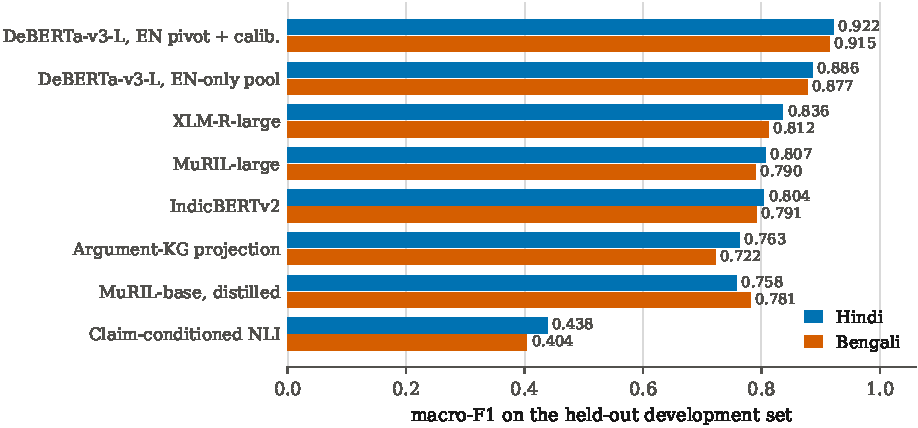
\includegraphics[width=\linewidth]{figures/fig_results.pdf}
\caption{Held-out development macro-F1 by system. The two highest bars are
English-pivot models; every native-script encoder, including three large ones,
falls below them.}
\label{fig:results}
\end{figure}

Before adopting a gain of that size we verified that it was not leakage. The
English distillation pool shares zero (language, identifier) keys with the
development set, no development comment text appears verbatim in any training
text, and the GWSD and SemEval pool contains no evaluation comments at all.

\paragraph{Component contributions.}
Calibration is worth $+0.019$ to $+0.023$ on the pivot channel and $+0.04$ to
$+0.08$ on base encoders. Model scale is worth $+0.05$ to $+0.08$: MuRIL-base
to MuRIL-large, and XLM-R-base at $0.717$ to XLM-R-large at $0.836$. The
auxiliary node head and the soft-label term are both retained in the submitted
configuration.

\paragraph{Submitted runs.}
Both language files carry the calibrated English pivot as the primary
classifier, the English-pool DeBERTa variant as the second, and XLM-R-large on
native script as the third. All three are trained classifiers. The three
columns agree on $87.2\,\%$ of Hindi comments and $86.4\,\%$ of Bengali
comments.

%% ---------------------------------------------------------------------------
\section{Negative and Methodological Results}
\label{sec:negative}

\paragraph{More in-distribution labels hurt.}
Refitting the distilled encoder on all 971 judge labels, rather than the 727
that exclude the development set, made it \emph{worse}: $0.655$ on Hindi and
$0.684$ on Bengali against $0.758$ and $0.781$, despite then training on the
very rows it was scored against. The likely cause is checkpoint selection.
With an internal early-stopping split drawn from a pool that is $92\,\%$
synthetic and translated text, the selected epoch is chosen against the wrong
distribution. More data is not automatically better when it changes what one
early-stops on.

\paragraph{Every ensemble lost to the best single model.}
Measured against the calibrated pivot, all tested blends were worse, from
$-0.009$ to $-0.035$, with most winning $0\,\%$ of 300 splits. With roughly
120 development rows per language, combination weights cannot be estimated
reliably, and a single strong model is the safer choice. We report this
because ensembling is the default expectation in shared-task submissions.

\paragraph{Unpaired strategy comparison is misleading.}
Our strategy selector initially ranked configurations by mean held-out
macro-F1 over independently drawn half-splits. Re-evaluated on identical
splits, one apparent Hindi gain of $+0.015$ shrank to $+0.005$, and an
apparent Bengali gain of $+0.023$ \emph{reversed sign} to $-0.002$. At this
data size any ensembling decision must be made on paired differences over
shared splits.

\paragraph{An evaluation-harness bug nearly cost us the best system.}
Our trainer's in-training development score for the English pivot read
$0.574$, and a retry read $0.331$, so we briefly abandoned the idea. Both
figures were artefacts: the harness evaluated using a text column that held
the Indic original, so an English-only model was being scored on Devanagari
input. The prediction path had been correct throughout. We report this because
the failure mode---a silent column mismatch producing a plausible-looking low
score rather than an error---is easy to reproduce and hard to notice.

%% ---------------------------------------------------------------------------
\section{Error Analysis}

The submitted system's weakest class is \textsc{None} in both languages
($0.870$ and $0.863$, against $\geq 0.96$ for \textsc{Against}). This matches
where the taxonomy predicted difficulty. \textsc{None} is not a semantic
category but the absence of a stance, and it collects channel praise,
questions, neutral facts and ambivalence---categories whose boundary with
\textsc{Favour} rests on a codebook decision rather than on the text. The most
frequent confusions are \textsc{None} predicted as \textsc{Favour}, where
polite engagement is read as agreement, and \textsc{Against} predicted as
\textsc{Favour}, where sarcasm survives translation poorly.

The most frequent arguments assigned by the panels were demands for action,
science-unreliable, attacks on the messenger, and channel praise. That
attacks on the messenger ranks fourth in Bengali is a direct vindication of
adding that node after the measurements of Section~\ref{sec:forensics}.

%% ---------------------------------------------------------------------------
\section{Limitations}
\label{sec:limitations}

\paragraph{Development labels are not human gold.}
This is the most important caveat. Our 244 development labels come from the
judge panel, so every figure in Table~\ref{tab:main} measures agreement with
that panel rather than with ground truth. The panel's internal agreement is
high ($\kappa = 0.859$) and a human reader reviewed and endorsed a
fifteen-comment sample, but that review was not blind and therefore yields no
independent agreement statistic. If the panel's reading of the \textsc{None}
boundary differs systematically from the organisers', our official score will
be lower than reported here, and our calibration---fitted to the panel's class
priors---may transfer imperfectly. We regard a blind human annotation of
50--150 comments as the single highest-value extension of this work.

\paragraph{The pivot requires machine translation at inference.}
The primary run consumes back-translated English. The classifier itself is a
local checkpoint with no API dependency, but reproducing the run requires
either the back-translated files, which we release, or a re-translation step.
Machine translation is a standard and organiser-encouraged step for this task,
but it is a pipeline dependency and we state it plainly.

\paragraph{Synthetic data reflects model priors.}
The 1\,040 generated comments encode a language model's \emph{model} of
Indian climate discourse, which is not the same thing as that discourse.

\paragraph{Small development set.}
Roughly 120 rows per language. All ensembling conclusions are correspondingly
weak, which is itself one of our findings.

%% ---------------------------------------------------------------------------
\section{Conclusion}

The lesson we would carry to another cross-lingual shared task is procedural:
measure the evaluation distribution before choosing a transfer strategy. Here
the nominal problem was Hindi and Bengali social media, the actual problem was
translated English, and recognising that was worth more than every
architectural choice we made combined. The argument taxonomy, the synthetic
corpus and the panel labels are released so that the components can be reused
and, where we were wrong, corrected.

%% ---------------------------------------------------------------------------
\section*{Declaration on Generative AI}

The author declares the following uses of generative artificial intelligence
in this work.

\emph{In the research pipeline}, generative AI is a studied component rather
than an incidental aid, and its role is described in full in
Sections~\ref{sec:synth}--\ref{sec:distil}. Specifically: large language
models generated the 1\,040-comment synthetic training corpus; a five-model
teacher panel and a three-model judge panel produced the pseudo-labels
distilled into the submitted classifiers and the development labels used for
calibration; and language-model-based machine translation produced the
Hindi and Bengali training translations and the English back-translations on
which the primary submitted run operates. No organiser-provided gold label was
used at any point. The limitations of relying on model-generated development
labels are stated in Section~\ref{sec:limitations}.

\emph{In preparing this manuscript}, the author used an AI assistant for code
implementation, experiment orchestration, and drafting and editing of the
text. All experimental design decisions, the forensic analysis, and the
interpretation of results are the author's own; the author verified all
reported numbers and takes full responsibility for the content of the
publication.

%% ---------------------------------------------------------------------------
\bibliography{referenences}

\end{document}
